\section{Nebenschlussgenerator}
Bei diesem Generatortyp liefert der Generator selbst den Erregerstrom zum Feldaufbau, da die Erregerwicklung parallel geschaltet wird (siehe Abbildung \ref{abb:neben_BKL_Messschaltung}). Zum Anlaufen ohne externe Spannung wird die Remanenz ausgenutzt, dabei ist bei der Verschaltung der Wicklung auf eine positive Rückkopplung zu achten, da sonst der vom Erregerstrom $I_E$ erregt Fluss $\Phi$ die zum Remanenzfluss $\Phi_R$ entgegengesetzte Polarität aufweist, ihn somit schwächt, sodass der Selbsterregungsprozess nicht zustande kommt. Dies kann sogar zur Entmagnetisierung der Maschine führen, worauf für ein erneutes Anfahren eine fremde Erregung benötigt wird.\\

\subsection{Äußere Kennlinie}
\begin{figure} [htb]
    \centering
    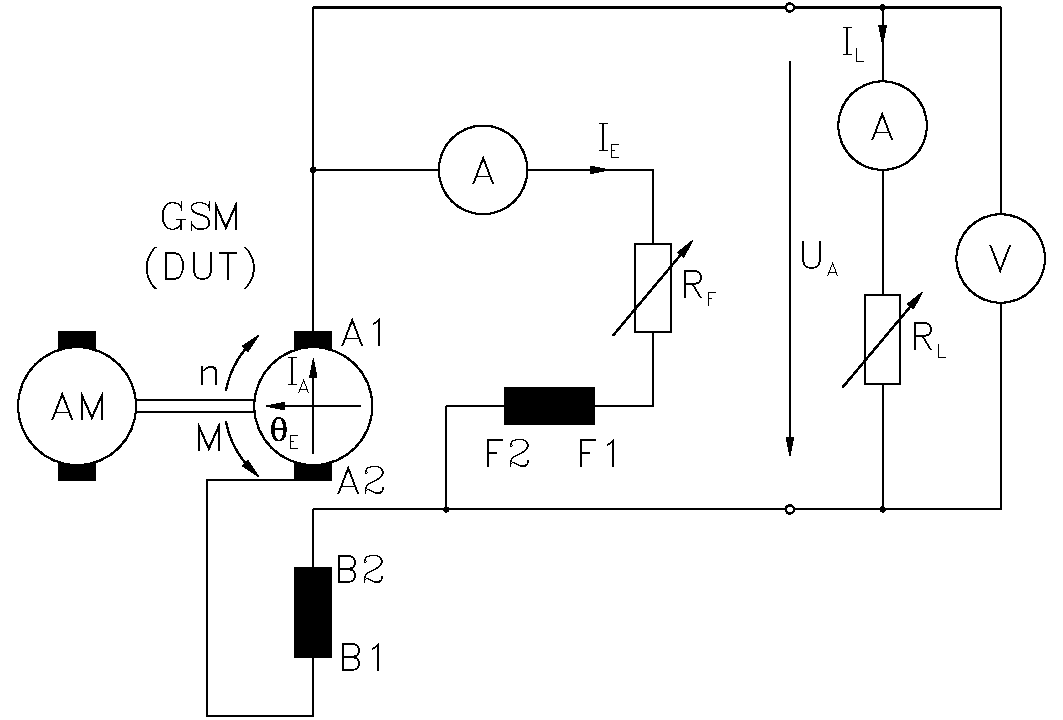
\includegraphics[width=0.55\textwidth, angle=0]{\currfiledir images/Belastungskennlinie_nebenerregt}
    \caption{Messschaltung zur Ermittlung der äußeren Kennlinie des Nebenschluss\-gleich\-strom\-generators (GSM).}
    \label{abb:neben_BKL_Messschaltung}
\end{figure}
\noindent Bei der Äußeren Kennlinie wird der Verlauf der Ausgangsspannung $U_A$ in Abhängigkeit der Belastung, d.h. des Ausgangsstromes $I_L$ ermittelt.\\
Dazu wird die Gleichstrommaschine wieder über die Antriebsmaschinen auf Nenndrehzahl $n=n_N$ beschleunigt und gehalten.\\
Der Startpunkt der Messung wird über die Widerstände $R_L$ und $R_F$ so gewählt, dass sich für einen Felderregerstrom $I_E=\SI{1.65}{\ampere}$ eine Ausgangsspannung $U_A=\SI{200}{\volt}$ einstellt. Anschließend wird die Belastung reduziert, d.h. der Widerstand $R_L$ erhöht, bis sich der Erregerstrom auf $\approx1.2\,I_{E,N}$ erhöht. Um den Einfluss der Hysterese zu minimieren, wird bei der folgenden Kennlinienaufnahme, die Belastung stets erhöht, d.h. der Widerstand $R_L$ kontinuierlich verringert.\\
Die daraus erhaltene äußere Kennlinie des Nebenschlussgenerators ist in Abbildung\;\ref{abb:nebenschluss_aussen} ersichtlich.\\
Im Vergleich zur äußeren Kennlinie des fremderregten Gleichstromgenerators (siehe Abb.\;\ref{abb:fremd_aussen_regulier}, Ankerspannung $U_A$), ist vor allem die stärkere Abhängigkeit der Ausgangsspannung $U_A$ vom Ausgangsstrom $I_A$ offensichtlich.\\
Bei Belastung sinkt durch den ohmschen Spannungsabfall am Ankerwiderstand $R_A$ die Ankerspannung. Dadurch sinkt auch die an der Nebenschlusswicklung anliegende Spannung und damit der von ihr getriebene Erregerstrom $I_E$ und somit der Fluss, sodass die Ankerspannung stärker sinkt als beim fremderregten Generator (konstante Erregerspannung). D.h. die Ausgangsspannung des Nebenschlussgenerators sinkt überproportional mit steigendem Ausgangsstrom, d.h. stärker als der ohmsche Spannungsabfall am Ankerwiderstand (vgl. Abb.\;\ref{abb:fremd_aussen_regulier}) es vermuten lässt.\\
Schließlich tritt aufgrund der fehlenden Kompensationswicklung bei sehr hohen Ankerströmen, die Ankerrückwirkung in Form einer globalen Feldschwächung in Erscheinung. Durch das geschwächte Hauptfeld wird weniger Spannung in die Maschine induziert, was eine weitere Reduktion der Ankerspannung nach sich zieht.\\
Wird die Maschine noch stärker belastet, so wird ein Punkt der Kennlinie erreicht, ab dem durch eine weitere Reduktion des Lastwiderstandes keine Erhöhung des Ausgangsstromes mehr erreicht werden kann. Der Erregerstrom und damit das Feld und schließlich die Ankerspannung, nehmen soweit ab, dass auch der Ausgangsstrom wieder zu sinken beginnt.\\
Der Kurzschlusspunkt des Generators stellt sich bei kurzgeschlossenem Ausgang ein (Felderregerstrom $I_E=0$), wobei aufgrund des Remanenzflusses $\Phi_R$ in der Maschine zumindest die Remanenzspannung $U_R$ induziert wird. Der Ausgangsstrom $I_L$ aus dem Generator wird durch den Ankerwiderstand begrenzt.\\
Der Kurzschlusspunkt konnte aufgrund des Mindestwertes des verwendeten Lastwiderstandes nicht erreicht werden.\\
Aufgrund der Erwärmung der Maschine während der Messung, ergibt sich der nicht-ideale Verlauf der Kurvenform (Dellen).
\input{\currfiledir Nebenschluss}
%\input{\currfiledir schaltung}